\documentclass[a4paper]{fhnwreport}

\graphicspath{{./graphics/}{./Bilder/}}

\title{Kurzanleitung \textsc{Detroit Electric Car}}
\author{Yanick Frei}
\date{\today}

\begin{document}
\begin{Large}
\setlength{\itemsep}{20pt}

\maketitle
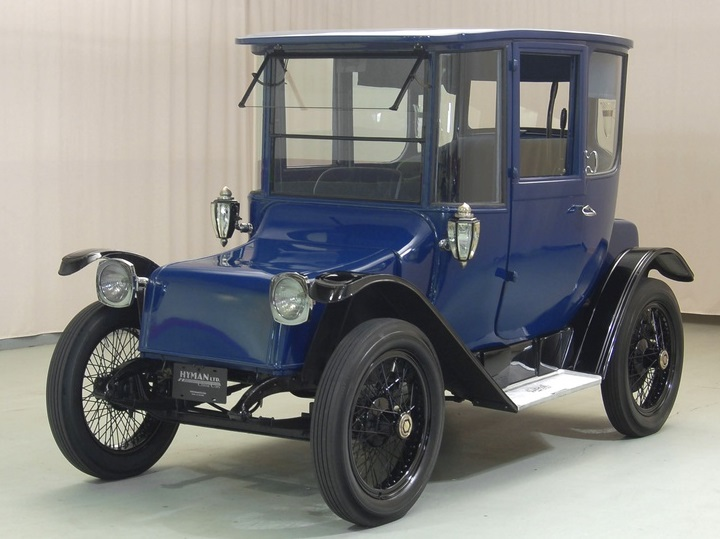
\includegraphics[width=1.00\textwidth]{Titelbild.jpg}

\newpage

In diesem Dokument soll kurz auf den \textsc{Detroit} eingegangen werden, insbesondere auf dessen Bedienung. Für weitere Informationen, insbesondere fachliche Fragen, sei auf den Fachbericht zum Umbau des Fahrzeuges verwiesen. Wir wünschen nun viel Spass beim Lesen und vor allem beim Fahren!

\tableofcontents \newpage

\section{Informationen zum Fahrzeug}

\section{Aufladen den Batterie}
Das Aufladen der Batterie geschieht in mehreren Schritten (\textit{kursive} Vorgänge werden dabei automatisch von der Batteriesteuerung übernommen):

\begin{enumerate}
\setlength{\itemsep}{10pt}
	\item Das Fahrzeug wird abgestellt und im Idealfall mit der Handbremse gesichert.
	\item Das 230V-Ladekabel wird eingesteckt und an der Steuerbox der Schalter auf \textsc{Ein} geschaltet.
	\item \textit{Das 12V-Netz des Fahrzeuges wird automatisch unterbrochen, womit der Hauptschalter nicht mehr eingeschaltet und losgefahren werden kann. Das soll ein versehentliches Losfahren während dem Laden verhindern.}
	\item \textit{Sind die Batterien nicht voll, wird automatisch der Ladephase gestartet. Bei komplett entleerter Batterie kann diese Phase bis zu 10 Stunden dauern.}
	\item \textit{Bereits während der Ladephase beginnt die Balancingphase, welche eine gleichmässige Ladung der Zellen sicher stellt. Diese Phase sollte im Normalfall nicht viel länger dauern als die Ladephase (das finale Balancing kann erst nach dem Vollladen der Zellen durchgeführt werden)}
	\item Nach dem Entfernen des Netzkabels wird das 12V-Netz wieder freigegeben, was ein Einschalten des Fahrzeugs ermöglicht.
\end{enumerate}

Der gesamte Ladevorgang inklusive Balancing sollte im Normalfall höchstens 12 Stunden dauern (bei komplett leerer Batterie). Das Ende der Ladephase kann einfach dadurch erkennt werden, dass beide Ladegeräte in der Front des Fahrzeugs ihre Lüfter abgestellt haben. Wenn möglich sollte ab dann der Balancingphase noch zwei Stunden Zeit gegeben werden. Falls dies nicht möglich ist, kann dies jedoch auch durch eine längere Balancingphase beim nächsten Ladevorgang kompensiert werden.

\section{Bewegen des Fahrzeuges}

\section{Bekannte Schwachstellen}


\end{Large}
\end{document}